\documentclass[11pt]{article}

\usepackage[margin=1.1in]{geometry}
\usepackage{amsmath,amssymb}
\usepackage{graphicx}
\usepackage{booktabs}
\usepackage{microtype}
\usepackage{xcolor}
\definecolor{linkblue}{rgb}{0.0,0.2,0.55}
\usepackage[colorlinks=true,linkcolor=linkblue,citecolor=linkblue,urlcolor=linkblue]{hyperref}

\newcommand{\Nsat}{N_{\mathrm{sat}}}
\newcommand{\CELL}{\mathrm{CELL}}

\title{A packing model of a closed universe:\\
random sequential adsorption of unit-rapidity worldlines\\
on a comoving torus}

\author{Chris Bentley \and Kevin Bentley}
\date{July 6, 2026}

\begin{document}
\maketitle

\begin{abstract}
We define and study a model universe built from nothing but mutually avoiding
worldlines. Each worldline is a closed path over a conformal time loop
$z \in (0,\pi)$, expressed per spatial axis as a sinusoidal expansion whose
non-trivial frequency components jointly obey a unit \emph{rapidity}
constraint $\sum_{k \ge 2} |k\,a_k| = 1$ (a built-in speed of light), while
the frequency-1 amplitude is a free comoving coordinate --- a separation that
makes homogeneity a property of the measure rather than an assumption.
Comoving space is a torus: a path leaving through one face re-enters through
the opposite one, so there is no boundary and no statable center. Even
frequencies carry a free phase; odd frequencies are shown to already possess
their full phase freedom. Packing these worldlines by random sequential
adsorption under an everywhere-in-time exclusion rule produces a jam whose
count grows as a clean power law $\Nsat \sim T^{D}$ in the time resolution
$T$, with $D = 2.33$ in three spatial dimensions and $1.38$--$1.40$ in two
--- strictly below the spatial dimension, yet demonstrably not the fractal
dimension of any static set: the equal-time slices of the jam are
\emph{exactly} uniform (wrapped correlation dimension $3.01$ and $2.03$; rms
comoving spread flat at $\sqrt{1/3}$ over the entire loop), and the worldline
bundle's local dimension sweeps from $1$ to $d$ with no plateau at $D$. The
model makes a parameter-free kinematic prediction: mover velocities at
maximum expansion should follow the arcsine law $P(v) = 2/\pi\sqrt{1-v^2}$,
diverging integrably at the speed cap. The packed state inherits the law's
shape --- including the relativistic pile-up at $v \to 1$ --- but with a
measurable tilt toward slow movers ($\langle v^2\rangle = 0.40$ vs the
proposal's $0.50$): jamming \emph{selects on phase}. The resulting equation
of state at the turnaround is matter-like, $w = 0.070$, flat across the
entire resolution ladder and identical under two independent energy
dictionaries. We close with the geometry of what remains unexplored ---
multi-frequency worldlines, intersecting ``unique groups'' and their
subpaths --- and with a discussion of whether the jam supports a
strange-attractor reading.
\end{abstract}

\section{Introduction}

Most model universes start from fields on a background. This one starts from
\emph{paths}. The only objects in the model are worldlines --- closed
trajectories through a finite expanding-and-contracting spacetime --- and the
only law is that they may not intersect. ``Matter'' is whatever set of
worldlines survives being packed, one at a time and at random, until nothing
more fits. The questions one can ask of such a universe are correspondingly
concrete. How much fits? What does the surviving population look like ---
where is it, how fast does it move, what microscopic traits did the packing
select for? And do any of the answers resemble physics?

The packing problem itself belongs to a classical family: random sequential
adsorption (RSA), the irreversible random placement of mutually excluding
objects, exactly solvable in one dimension \cite{renyi} and much studied
since for compact shapes \cite{evans,torquato}. Our objects are not compact.
A worldline must avoid every other accepted worldline at \emph{every} moment
of the loop simultaneously, so the excluded volume seen by a candidate is a
joint, global object --- and this, it will turn out, is where all of the
model's nontrivial structure lives.

This paper does three things. First, it defines the model carefully
(Section~\ref{sec:model}): the worldline family, the rapidity constraint that
plays the role of a speed of light, the toroidal comoving space that removes
any preferred center, the phase freedom of even frequencies, and the
intersection rules --- including the notions of \emph{unique groups} and
\emph{subpaths}, which define how the model is meant to be filled beyond the
sector explored here. Second, it reports what has been measured in the first
explored sector --- worldlines with a single wiggle frequency per axis, one
path per group --- packed at scale on GPU hardware
(Sections~\ref{sec:method}--\ref{sec:kinematics}): the growth exponent of the
jam, the exact homogeneity of its slices, the absence of a geometric carrier
for the exponent, the parity structure of the surviving frequencies, an
arcsine velocity law with a measured deviation that quantifies how jamming
selects on phase, and a resolution-independent, dictionary-robust equation of
state. Third, it discusses what the results do and do not license one to
conclude --- including the question of whether the jam is usefully described
as a strange attractor --- and lays out the unexplored territory
(Section~\ref{sec:disc}).

We have tried to keep the presentation self-contained and readable rather
than maximally terse; where a derivation is short we give it, and where a
claim is speculative we say so. All code (packing engines, orchestration,
analysis), all data, and a dated lab notebook are public.\footnote{%
\url{https://github.com/universe-analysis/universe-generator}.}

\section{The model}
\label{sec:model}

\subsection{Worldlines as constrained sinusoidal expansions}
\label{sec:worldlines}

Time is a coordinate $z \in (0,\pi)$, and the universe carries a scale factor
$a(z) = \sin z$: it expands from a bang at $z = 0$ to a maximum at the
turnaround $z = \pi/2$ and recontracts to a crunch at $z = \pi$. Along each
spatial axis, a worldline is a superposition of integer-frequency sine terms,
\begin{equation}
  x(z) \;=\; a_1 \sin z \;+\; \sum_{k \ge 2} a_k
  \bigl[\sin(kz + f_k) - \sin f_k\bigr],
  \qquad k \in \mathbb{Z},
  \label{eq:general}
\end{equation}
subject to three structural rules.

\paragraph{Closure.} The path must begin and end at zero: every worldline
meets the bang and the crunch. The subtracted constants $\sin f_k$ in
Eq.~\eqref{eq:general} enforce this in the presence of phases --- each
component is re-pinned to zero at the endpoints. Closure is also why phases
are restricted as they are below.

\paragraph{The rapidity constraint.} All frequency components except $k=1$
jointly obey
\begin{equation}
  \sum_{k \ge 2} |k\, a_k| \;=\; 1 .
  \label{eq:rapidity}
\end{equation}
Since each term contributes at most $|k a_k|$ to $|dx/dz|$, this is a unit
speed budget --- a speed of light built into the family rather than imposed
on it. A worldline with $0.5\sin 2z$ spends its whole budget
($0.5 \times 2 = 1$); one with $\tfrac{1}{5}\sin 3z + \tfrac{1}{5}\sin 2z$
spends $\tfrac{3}{5} + \tfrac{2}{5} = 1$ likewise. The amplitudes of all
non-trivial components are thus dependent on one another: speed spent on one
frequency is unavailable to the rest.

\paragraph{The free comoving coordinate.} The $k=1$ amplitude is exempt from
the budget and drawn freely, $a_1 \in (-1,1)$. This term has a special
meaning: in \emph{comoving} coordinates $X = x/\sin z$ it is simply the
constant $a_1$ --- a static comoving position, the Hubble flow. Separating it
from the rapidity constraint is what erases the preferred center: position
costs nothing, so a uniform draw of $a_1$ is exactly the homogeneous measure,
and nothing in the dynamics couples where a worldline sits to how fast it may
move. (Section~\ref{sec:homog} shows the packing preserves this
homogeneity exactly.)

\paragraph{Phases.} Even frequencies may be freely modulated by a constant
phase $f_k \in [0,\pi)$. Odd frequencies carry no explicit phase --- and need
none: for odd $k$, a sign flip of the amplitude is exactly a phase shift by
$\pi$ ($\sin(kz + \pi) = -\sin kz$ and the closure offset transforms
consistently), and this is the entire phase freedom compatible with closure,
since $\sin(k\pi + f) = \pm \sin f$ cancels the re-pinning constant only when
$k$ is even. Odd components are, in this sense, already modulated to the
highest allowable degree; even components acquire a genuinely new continuous
degree of freedom. This asymmetry between the parities threads through
everything that follows.

The frequencies $k$ range over all positive integers in the abstract model.
Under discrete analysis (Section~\ref{sec:discrete}) the timestep resolution
imposes a Nyquist ceiling, which is the only place a frequency cutoff enters.

\subsection{Comoving space is a torus}
\label{sec:torus}

The bounds of the universe along each axis are the curves $\pm\sin z$ --- the
envelope traced by the extremal $k = 1$ worldlines. A path that crosses
$+\sin z$ does not end or reflect: it re-enters at $-\sin z$ moving toward
the center it just left. In comoving coordinates this is the statement that
$X$ lives on a circle of circumference 2, with $X = +1$ and $X = -1$ the
same point; with $d$ spatial axes, comoving space is a $d$-torus. Distances
(and hence intersections) are computed in the minimum image. Two structures
that a bounded model would possess are thereby not removed but rendered
\emph{unstatable}: there is no wall, and no point is distinguishable as a
center.

\subsection{The spacetime view}

A full worldline in $d{+}1$ dimensions is the parametric curve
\begin{equation*}
  \bigl(x_1(z),\, \ldots,\, x_d(z),\, z\bigr), \qquad z \in (0,\pi),
\end{equation*}
with an independent expansion~\eqref{eq:general} per axis: a $d$-dimensional
path unfolding over time. All results in this paper are for $d = 2$ and
$d = 3$ (``$2{+}1$'' and ``$3{+}1$''). It is worth noting what the family
\eqref{eq:general} is, seen whole: since every closed path with bounded
velocity admits a sine expansion, the model with all frequencies admitted is
(a discretization of) the space of \emph{all} closed unit-rapidity paths on
the loop --- the single-frequency sector studied below is its first, sparsest
slice.

\subsection{Intersections, unique groups, and subpaths}
\label{sec:groups}

Two worldlines \emph{intersect} if they come within the exclusion distance of
each other (made precise in Section~\ref{sec:discrete}) at any moment of the
loop. The organizing notion of the model is the \emph{unique group}: a set of
paths that each intersect at least one other member of their own group and
never intersect any path of another group. A unique group with several member
paths is one object that exists in several places at once; a group with a
single path is the degenerate case.

The intended construction of a full universe proceeds in two stages. First,
fill the loop with mutually non-intersecting paths --- every group a
singleton --- until jamming (or any chosen earlier stopping point). Second,
continue filling by adding \emph{subpaths}: new paths that intersect a member
of an existing group (thereby joining it) while still avoiding all other
groups. The first stage is a hard-sphere-like packing problem; the second
redistributes the remaining room among the existing identities rather than
creating new ones.

Everything measured in this paper concerns the first stage. Subpaths, and
worldlines carrying more than one budget frequency, are defined by the model
but not yet explored; we return to what questions they open in
Section~\ref{sec:disc}, and we deliberately draw no conclusions about them
here.

\subsection{Discrete analysis: timesteps, Nyquist, exclusion}
\label{sec:discrete}

Analysis proceeds at a chosen \emph{resolution} $T$: the loop is sampled at
$T$ evenly spaced interior times $z_i = i\pi/(T{+}1)$, $i = 1,\ldots,T$. The
resolution fixes everything else:
\begin{itemize}
  \item \textbf{Nyquist ceiling.} Frequencies are admitted up to $k \le T$
        --- beyond that a component cannot be resolved by the grid.
  \item \textbf{Exclusion.} Each path carries an exclusion radius of $1/T$
        in comoving coordinates (Chebyshev metric, minimum-image on the
        torus): two paths intersect if at any sampled time their comoving
        separation is below $2/T$ per axis. The exclusion cell shrinks
        exactly as the resolution grows, so ``how much fits at resolution
        $T$'' is a well-posed scaling question.
\end{itemize}
Packing is random sequential adsorption: candidates are drawn from the
measure described above (uniform $a_1$; frequencies from the admitted band
with a high-frequency bias and pairwise-coprime axis frequencies; signs and
phases uniform) and accepted iff they intersect no previously accepted path.
True jamming is logarithmically slow to reach at large $T$, so runs stop at
an acceptance-rate cutoff of $10^{-6}$ (one accepted candidate per million
attempts); the flatness of the measured local scaling slopes across the
ladder (Fig.~\ref{fig:jam}, lower panel) indicates the configurations are
well inside the scaling regime, and the extrapolation to literal jamming is
flagged as an open problem rather than assumed away.

\section{Generation at scale}
\label{sec:method}

The explored sector --- one budget frequency per axis, i.e.
$x(z) = a\,[\sin(bz + f) - \sin f] + a_1 \sin z$ with $|ab| = 1$ per axis ---
is packed by CUDA engines (one for each $d$). The engine's collision test
exploits a small identity: the exclusion threshold in physical coordinates is
$\sin(z_i)\cdot 2/T$, which in comoving coordinates collapses to the constant
$2/T$ at every timestep, so a uniform spatial hash with exactly $T$ cells per
axis per timestep gives an $O(NT)$ (rather than $O(N^2 T)$) test, wrapping
mod $T$ for the minimum image. Memory scales as $T^{d+1}$; consumer GPUs
reach $T = 200$ at $d = 3$ and $T = 400$ at $d = 2$. Campaigns are dispatched
over a small GPU fleet by a resumable orchestrator, and each accepted
worldline's parameters $(a, b, a_1, f)$ per axis are dumped, so any
configuration can be reconstructed analytically at any $z$ offline. The
datasets below are: $d = 3$, $T = 20$--$200$ in steps of 10, five seeds per
$T$; $d = 2$, $T = 40$--$400$ in steps of 20, eight seeds per $T$.

Four estimator families are used. The \emph{jam-count exponent} is the
weighted log--log slope of $\Nsat$ vs $T$ with seed-bootstrap errors, checked
for power-law quality via local pairwise slopes. The \emph{correlation
dimension} $D_2$ of an equal-time slice uses the Grassberger--Procaccia
integral \cite{gp} with both spherical ($L^2$) and cubic ($L^\infty$) probes;
because the domain is periodic, the correct estimator wraps distances
(minimum image; implemented with a periodic $k$-d tree), and we also report
the naive open-boundary estimator on the same clouds as a deliberate
control. \emph{Box-counting} of slices and of the full worldline bundle is
reported as local slope vs scale and used diagnostically (it converges far
too slowly in $T$ to serve as a headline estimator). Kinematic and
equation-of-state quantities are computed analytically from the dumped
parameters (Section~\ref{sec:kinematics}).

\section{How much fits: the jam-count exponent}
\label{sec:count}

\begin{figure}[t]
  \centering
  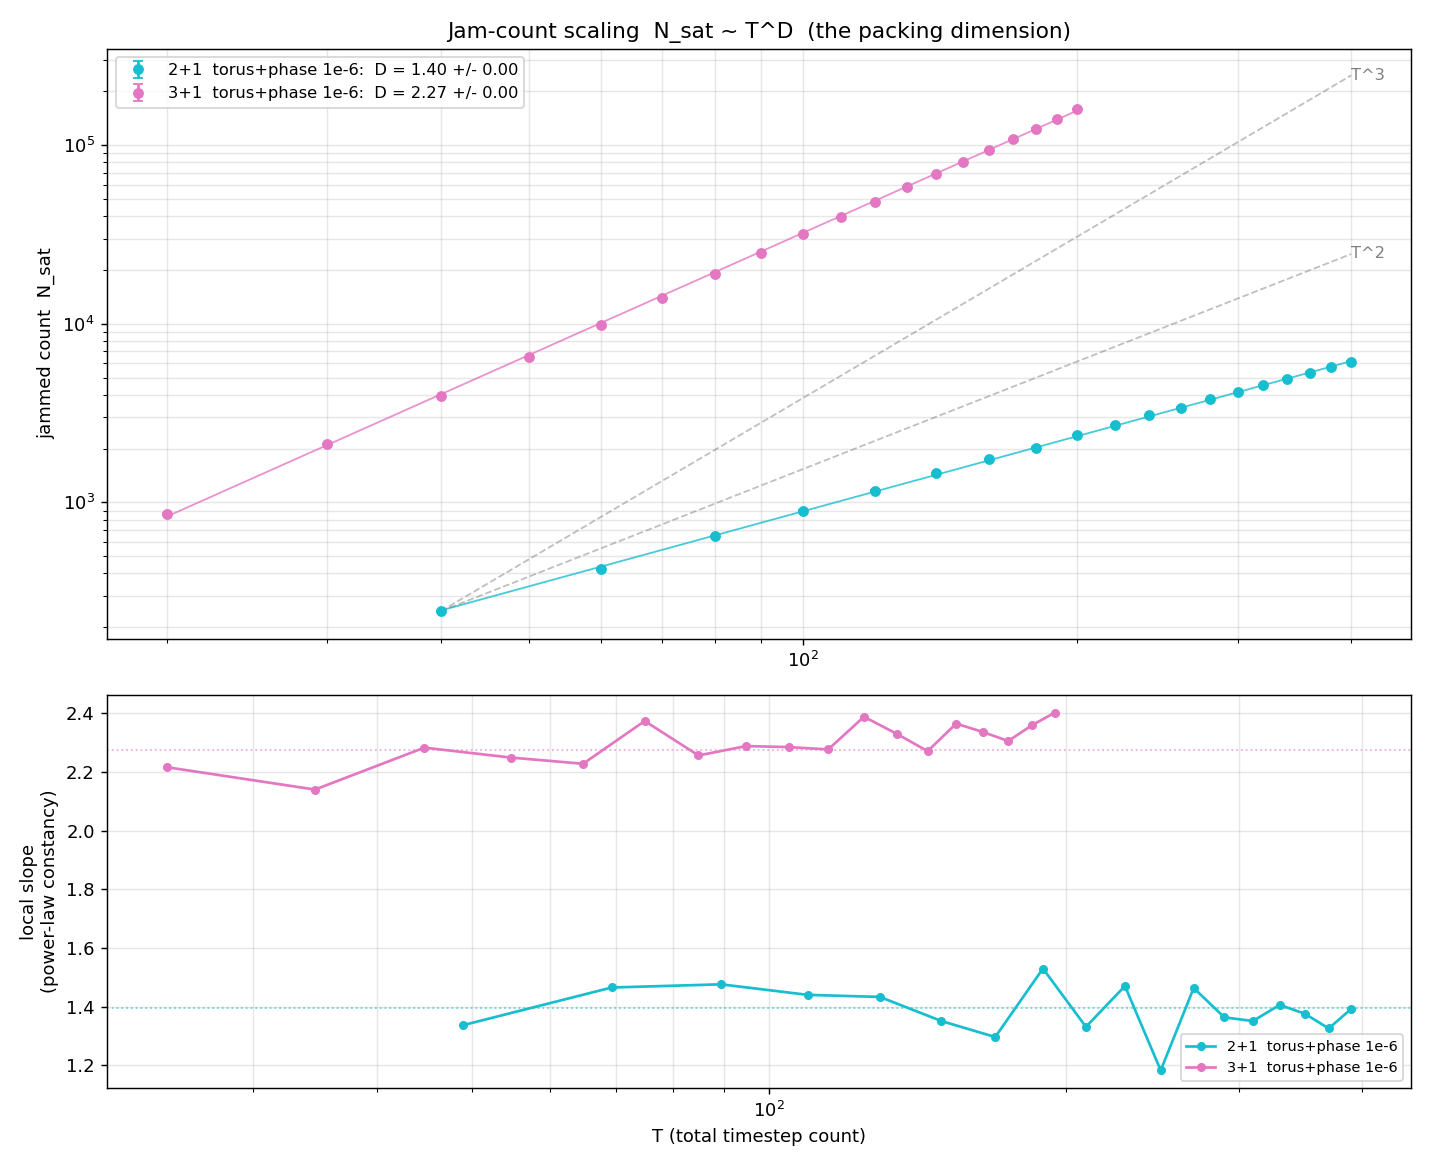
\includegraphics[width=\textwidth]{figs/jam_scaling.png}
  \caption{Jam count $\Nsat$ vs resolution $T$ (log--log) for the two
  explored dimensions, with $T^2$ and $T^3$ guides. Lower panel: local
  pairwise slopes --- flat across the ladder, i.e.\ clean power laws with no
  crossover. Fitted exponents: $D = 2.27$ (full ladder) rising to $2.33$ on
  the $T \ge 100$ half in $3{+}1$; $1.40$ full / $1.38$ high-$T$ in $2{+}1$.}
  \label{fig:jam}
\end{figure}

The jammed count is a clean power law, $\Nsat \sim T^D$, over the full
measured ladder in both dimensions (Fig.~\ref{fig:jam}):
\begin{equation*}
  D_{3+1} = 2.273 \pm 0.003 \ \text{(full ladder)}, \quad
  2.331 \pm 0.003 \ (T \ge 100);
  \qquad
  D_{2+1} = 1.396 \pm 0.002, \quad 1.375 \pm 0.004 .
\end{equation*}
Local slopes are flat (scatter $0.066$ in $3{+}1$, $0.080$ in $2{+}1$) with
the mild low-$T$ bend absorbed by the high-$T$ fits; we quote $D \approx
2.33$ and $D \approx 1.38$ as the converged values at this cutoff. At the top
of the ladders the jams hold $\langle\Nsat\rangle \approx 1.6 \times 10^5$
worldlines ($T = 200$, $d = 3$) and $6.1 \times 10^3$ ($T = 400$, $d = 2$).

The exponent sits well below the spatial dimension in both cases. Pure
spatial packing would give $\Nsat \sim T^d$: each path excludes $O(1)$ cells
of a $T^d$ comoving grid, and slices, as the next section shows, are packed
homogeneously. The deficit --- $T^{2.33}$ against a $T^3$ ceiling --- is
therefore not a matter of where the worldlines sit. It is the price of the
\emph{joint} constraint: a candidate must thread the gaps of every one of
$T$ time slices simultaneously, and the number of trajectories able to do so
grows more slowly than the room available in any single slice. We call $D$ a
\emph{packing-number exponent}, and Section~\ref{sec:notgeom} substantiates
the name by showing no static set carries it as a geometric dimension.

\section{Where it sits: exact homogeneity}
\label{sec:homog}

\begin{figure}[t]
  \centering
  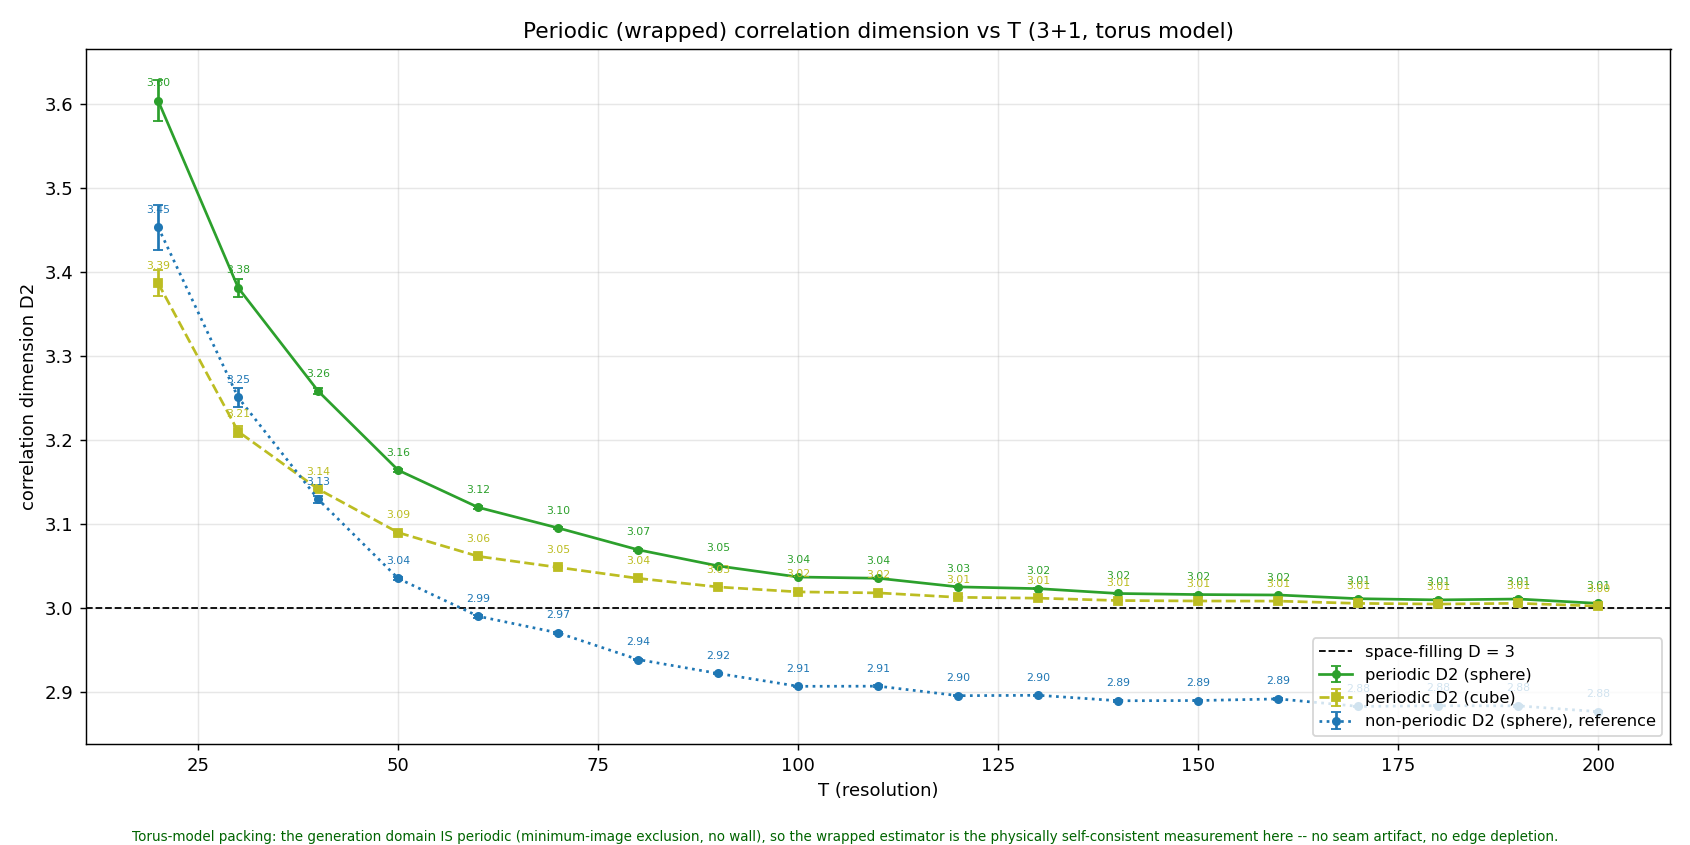
\includegraphics[width=\textwidth]{figs/wrapped_d2_3d.png}
  \caption{Wrapped (minimum-image) correlation dimension of the turnaround
  slice vs $T$ ($3{+}1$, five seeds per $T$): spherical and cubic probes
  converge together onto the space-filling $D = 3$ line ($3.01$ at
  $T = 200$). The open-boundary estimator on the same clouds (dotted) reads
  ${\sim}2.89$ --- the artifact a non-periodic estimator commits on periodic
  data, shown as a control.}
  \label{fig:wrapped}
\end{figure}

\begin{figure}[t]
  \centering
  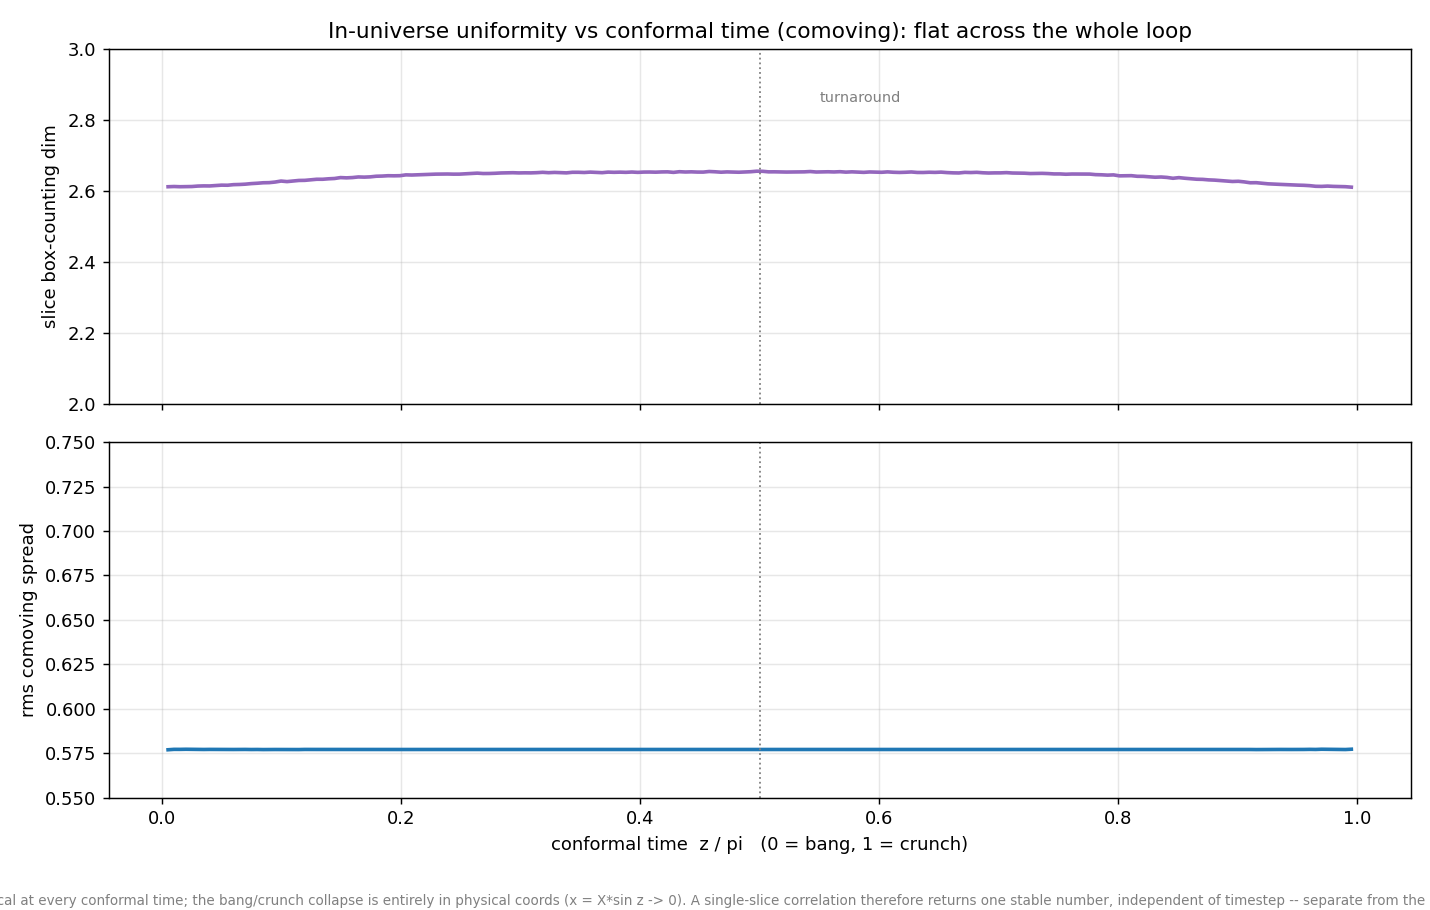
\includegraphics[width=\textwidth]{figs/uniformity.png}
  \caption{One universe over its whole history ($3{+}1$, $T = 200$, five
  seeds): slice box-counting dimension (top) and rms comoving spread
  (bottom) vs conformal time. The spread sits on $\sqrt{1/3}$ --- the exact
  uniform-torus value --- flat through bang, turnaround, and crunch.}
  \label{fig:uniformity}
\end{figure}

The matter distribution of the jam is exactly uniform, and this holds in two
senses. Across space: the wrapped correlation dimension of the turnaround
slice converges onto the space-filling value with the probe-shape gap
collapsed,
\begin{equation*}
  D_2 = 3.019 \ \text{(sphere)} \ / \ 3.010 \ \text{(cube)} \quad (d = 3),
  \qquad
  D_2 = 2.032 \ / \ 2.025 \quad (d = 2),
\end{equation*}
seed-averaged over $T \ge 100$ (Fig.~\ref{fig:wrapped}). Across time: fixing
one universe and scanning every conformal time, the rms comoving spread sits
at $\sqrt{1/3} \approx 0.5774$ --- the exact value for a uniform torus ---
flat across the entire loop, with the slice box-counting dimension confined
to a narrow band (Fig.~\ref{fig:uniformity}; its residual deficit from 3 is
the generic slow convergence of box-counting, not structure).

Homogeneity of the \emph{proposal} measure is built in --- that is what the
free comoving coordinate is for. The content of the measurement is that
\emph{jamming preserves it}: the exclusion interaction thins the population
by orders of magnitude without imprinting any density structure on the
survivors at any measurable scale, at any time. The bang/crunch collapse
lives entirely in the physical coordinates ($x = X \sin z \to 0$); the
comoving arrangement never knows it is happening.

One methodological remark, since it is easy to get wrong: the naive
correlation estimator (unwrapped positions, open-boundary distances) applied
to these same configurations reads $D_2 \approx 2.89$ ($d = 3$) and
$\approx 1.93$ ($d = 2$) with a spurious probe-shape split --- a boundary
artifact, reproduced deliberately in Fig.~\ref{fig:wrapped} as the dotted
control. On periodic data the wrapped estimator is not a refinement but the
definition; a uniform control cloud returns the exact ambient dimension
under it, for both probes.

\section{What the exponent is not: no geometric carrier}
\label{sec:notgeom}

\begin{figure}[t]
  \centering
  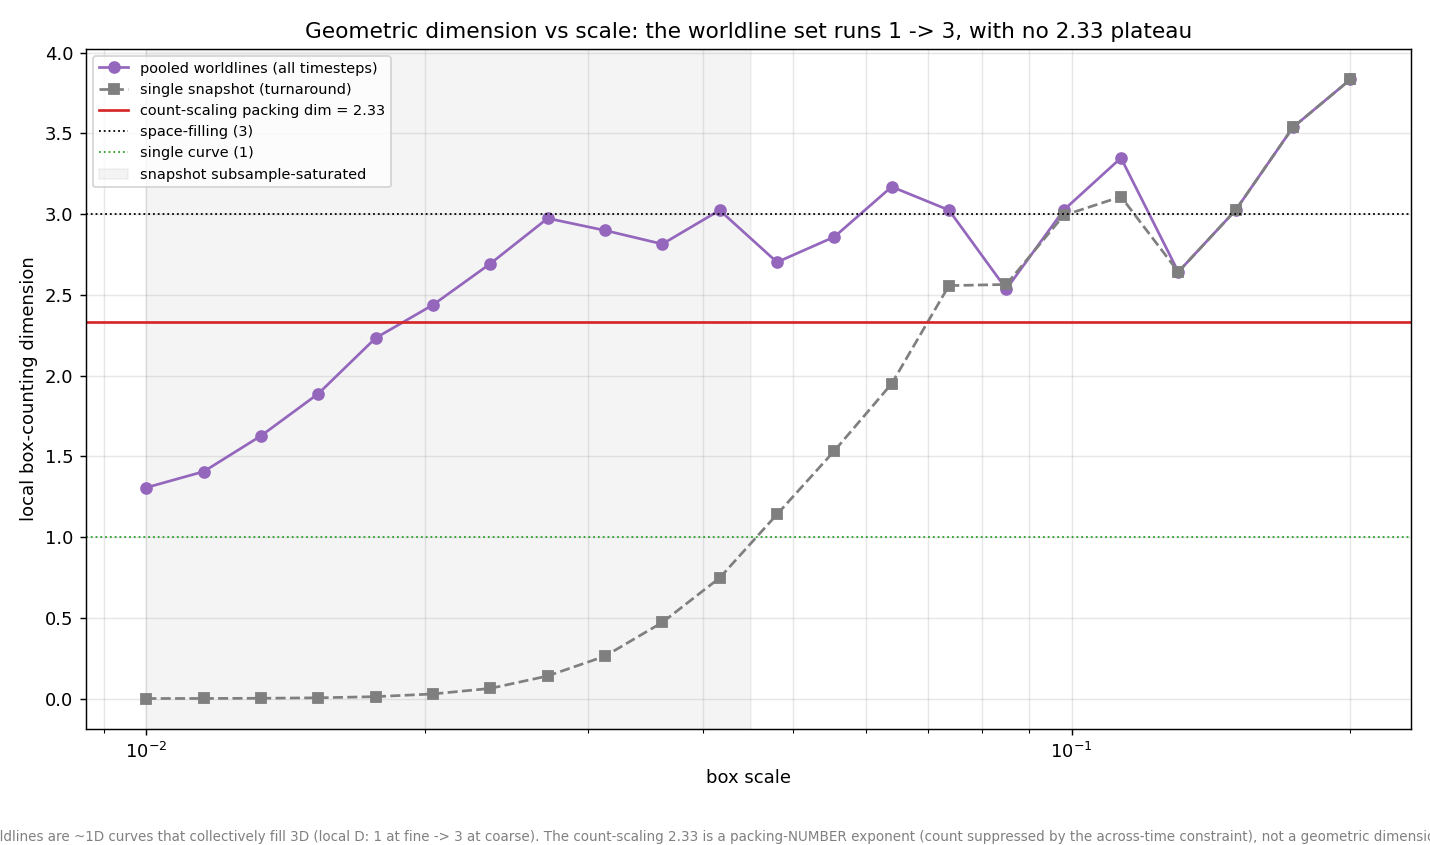
\includegraphics[width=0.95\textwidth]{figs/spacetime_boxdim.png}
  \caption{Local box-counting dimension vs scale for the pooled worldline
  bundle ($3{+}1$, $T = 200$, all timesteps pooled, three seeds). The local
  dimension sweeps from ${\approx}1.3$ near the packing cell (resolving
  individual smooth curves) through $2.76$ at intermediate scales to
  $2.89$ at coarse ones, crossing the count exponent $2.33$ (line) only in
  passing. No scale exhibits a plateau at $D$.}
  \label{fig:bundle}
\end{figure}

Given a sub-dimensional exponent, the natural reflex is to look for a fractal
--- some static set whose box or correlation dimension equals $2.33$. The
slices cannot be it: they are exactly three-dimensional
(Section~\ref{sec:homog}). The remaining candidate is the worldline bundle as
a whole, and it fails too (Fig.~\ref{fig:bundle}): pooling all timesteps of a
jam into one point cloud, the local box-counting dimension runs from
${\approx}1.3$ at the finest resolved scale --- where the cloud looks like a
union of smooth one-dimensional curves --- up to ${\approx}2.9$ at coarse
scales, where it is space-filling. It crosses $2.33$ in passing, with no
plateau; the same holds treating time as a fourth axis.

For packings of \emph{points}, packing number and box dimension coincide,
which is exactly why the reflex exists. For packings of extended curves under
a joint across-time constraint the two notions separate, and this model
separates them cleanly: geometry says ``uniform curves filling the space,''
counting says ``$T^{2.33}$ of them fit.'' The exponent measures a
\emph{dynamical} capacity --- how the number of globally non-intersecting
threadings scales with resolution --- and appears to have no static shadow.
We are not aware of a standard name for this quantity in the RSA literature.

\section{What survives: parity, the arcsine law, and the equation of state}
\label{sec:kinematics}

\subsection{Parity structure of the surviving frequencies}
\label{sec:parity}

\begin{figure}[t]
  \centering
  
\includegraphics[width=\textwidth]{figs/parity_vs_t.png}
  \caption{Composition of the jam vs resolution ($3{+}1$). Left: fraction of
  worldlines entirely odd-frequency vs carrying an even frequency. Right:
  fraction of all accepted frequencies that are odd. Both are flat above
  $T \approx 50$.}
  \label{fig:parity}
\end{figure}

\begin{figure}[t]
  \centering
  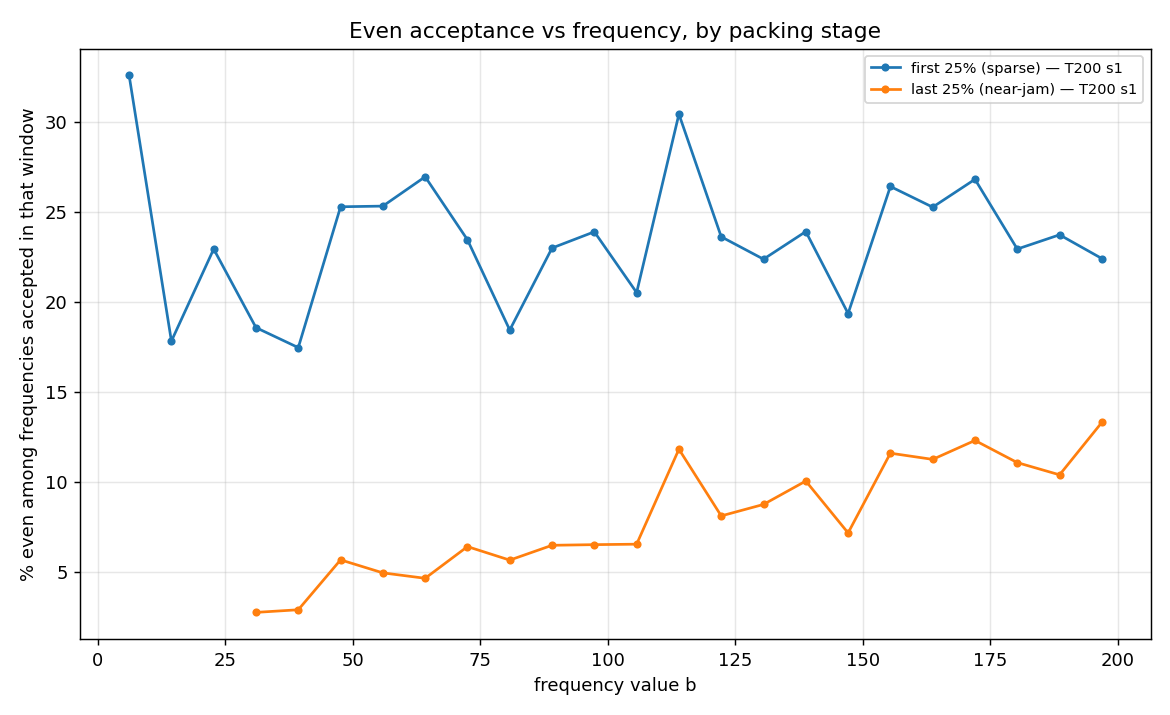
\includegraphics[width=0.8\textwidth]{figs/parity_stage.png}
  \caption{Even acceptance vs frequency value, resolved by packing stage
  ($3{+}1$, $T = 200$, a full ordered acceptance sequence of
  $N = 1.6\times10^5$ paths): first quartile of acceptances (sparse
  universe) vs last quartile (near jamming). The near-jam survivors skew
  strongly odd at every frequency.}
  \label{fig:stage}
\end{figure}

The comoving wiggle $\sin(bz+f)/\sin z$ is symmetric about the turnaround
when $b$ is odd (the worldline sits at a velocity extremum there --- at
rest) and antisymmetric when $b$ is even (it swings through at speed). The
jam has a definite, resolution-stable composition along this axis
(Fig.~\ref{fig:parity}): $48\%$ of packed worldlines are entirely
odd-frequency, and $82.7\%$ of all accepted frequencies are odd, both flat
in $T$ above ${\sim}50$. The pairwise-coprimality rule permits at most one
even frequency per worldline, so the population splits into a \emph{cold}
component (all odd, exactly at rest at the turnaround) and a \emph{mobile}
one (one even axis) --- and motion at maximum expansion is always
single-axis.

The selection is dynamical, not just distributional: resolving acceptance by
packing stage (Fig.~\ref{fig:stage}), even frequencies are accepted at
$20$--$27\%$ across the band while the universe is sparse, but among the
final quartile of survivors before jamming they are squeezed to $3$--$13\%$.
What still fits into the last gaps is overwhelmingly odd --- the objects
that hold still at the moment the universe is largest.

\subsection{A parameter-free speed law, and how jamming bends it}
\label{sec:arcsine}

The phase freedom of even frequencies turns the mobile component's
kinematics into a closed-form prediction. At the turnaround ($\sin z = 1$,
$\cos z = 0$) the peculiar velocity of an axis reduces to
\begin{equation}
  v \;=\; \bigl|\,a\,b \cos(b\pi/2 + f)\,\bigr|
    \;=\; |\cos f| \quad \text{for even } b
  \qquad (\text{and } v = 0 \text{ for odd } b),
  \label{eq:speed}
\end{equation}
using the rapidity constraint $|ab| = 1$. The free comoving term drops out
of the velocity entirely --- position and speed are independent by
construction. With the proposal phases uniform, $f \sim U[0,\pi)$, the speed
of a mover is arcsine-distributed:
\begin{equation}
  P(v) \;=\; \frac{2}{\pi\sqrt{1 - v^2}}, \qquad v \in [0,1),
  \qquad
  \langle v \rangle = \tfrac{2}{\pi}, \quad \langle v^2 \rangle = \tfrac12 .
  \label{eq:arcsine}
\end{equation}
This is a parameter-free law, and a physically suggestive one: the density
diverges (integrably) at the speed cap $v = 1$, a built-in relativistic
pile-up, while the cap itself is never exceeded.

\begin{figure}[t]
  \centering
  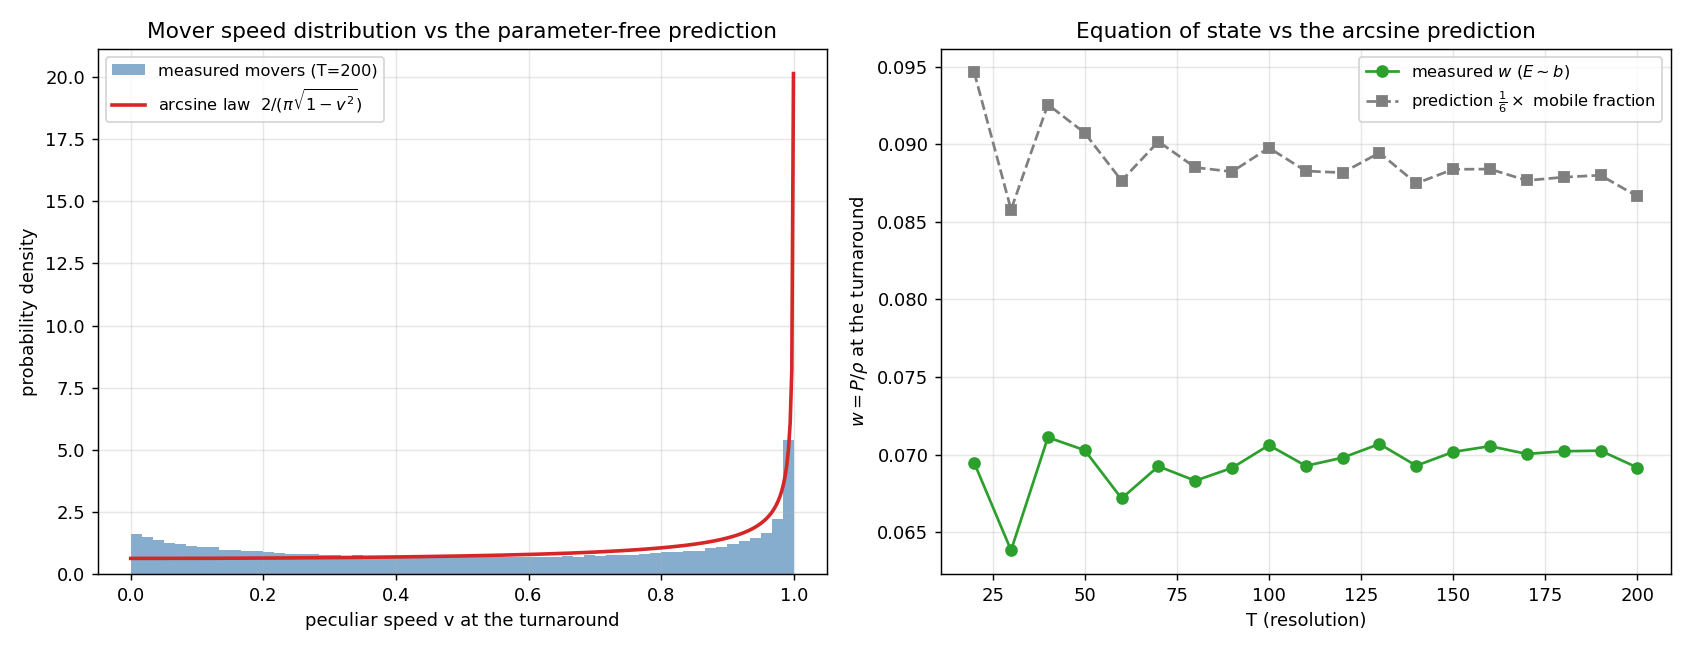
\includegraphics[width=\textwidth]{figs/phase_kinematics.png}
  \caption{Left: measured turnaround speed distribution of the mobile
  component ($3{+}1$, $T = 200$, $1.6 \times 10^5$ movers across five seeds)
  against the arcsine law of the proposal measure. The relativistic pile-up
  at $v \to 1$ survives packing, but attenuated, with a compensating excess
  of slow movers: jamming selects on phase. Right: the turnaround equation
  of state vs resolution --- flat at $w = 0.070$ across the entire ladder,
  ${\sim}20\%$ below the no-selection prediction
  $w = \tfrac{1}{6}\times(\text{mobile fraction})$.}
  \label{fig:kinematics}
\end{figure}

The packed state tells a sharper story (Fig.~\ref{fig:kinematics}, left).
The measured mover distribution keeps the arcsine shape qualitatively ---
including the pile-up against the cap --- but tilts: slow movers are
overrepresented and the cap spike is attenuated, with
\begin{equation*}
  \langle v \rangle_{\text{packed}} = 0.539 \ \ (\text{proposal } 0.637),
  \qquad
  \langle v^2 \rangle_{\text{packed}} = 0.404 \ \ (\text{proposal } 0.500).
\end{equation*}
Nothing in the acceptance rule references velocity; the tilt means that
\emph{jamming itself selects on phase}. A fast mover ($f$ near $0$ or
$\pi$) sweeps more comoving ground around the turnaround and is
correspondingly harder to thread through a crowded universe, so the
survivors' phases concentrate toward quadrature. This is selection acting on
a degree of freedom invisible to any single-time snapshot --- and it is
resolution-independent: the suppression factor is the same at every $T$
measured.

\subsection{The equation of state}
\label{sec:eos}

Assigning worldlines an energy $E$ and using the kinetic pressure of the
mobile component, $w = P/\rho = \tfrac13 \langle E v^2\rangle / \langle E
\rangle$, the turnaround equation of state is (Fig.~\ref{fig:kinematics},
right):
\begin{equation*}
  w \;=\; 0.070, \qquad \text{flat over the full ladder } (T = 20\text{--}200),
\end{equation*}
computed under $E \propto \sum_k b_k$ (a frequency/``wave'' dictionary) and
reproduced to $1\%$ under $E \propto$ arc length of the spatial path (a
``string'' dictionary): $0.0692$ vs $0.0700$ at $T = 200$. Both dictionaries
are parity-blind, and for any parity-blind $E$ the arcsine law predicts
$w = \tfrac16 \times (\text{mobile fraction}) \approx 0.087$; the measured
$w$ sits $20\%$ below it, which is precisely the phase-selection tilt of
Section~\ref{sec:arcsine} expressed thermodynamically. The universe at
maximum expansion is matter-like ($w \ll 1/3$), its pressure is carried by a
single-axis-moving minority whose speeds follow a tilted arcsine law, and
none of these statements depends on which of the two natural mass
dictionaries one adopts, nor on the resolution.

\section{Discussion}
\label{sec:disc}

\subsection{What kind of object is the jam?}

Assembling the measurements: the jam is spatially featureless at every
moment (exactly uniform slices, no center, no boundary, no fractality),
temporally featureless in comoving terms (statistically identical slices
across the loop), and yet strongly structured in every non-spatial
direction --- a sub-dimensional count exponent, a sharp parity composition,
a phase-selected velocity law, a definite equation of state. All structure
lives in the \emph{joint, whole-loop} character of the exclusion: which
trajectories can coexist, not where anything is.

Is the jam a strange attractor? The question is natural --- the toolset we
use (correlation integrals, generalized dimensions) comes from that field
\cite{gp,hp}, and the packing does exhibit attractor-like selection:
iterating acceptance drives the surviving population onto a measure-zero-ish
preferred subset of parameter space (odd-dominated frequencies, quadrature
phases, coprime tuples) that is stable across seeds and resolutions. But the
analogy has to be drawn in \emph{parameter space}, not physical space: the
spatial sets are exactly space-filling, so nothing strange lives there. What
would make the reading precise is currently open: one would want a
well-defined map whose iteration the RSA process approximates, evidence of
sensitive dependence (do neighbouring seeds diverge in composition?), and a
fractal measurement on the selected parameter-space set itself --- e.g.\ the
dimension spectrum of the accepted $(b, f, a_1)$ population --- none of
which has been done. We record the hypothesis and its test surface rather
than a claim.

A second reading of the count exponent deserves note: $D/d$ is
$0.78$ in $3{+}1$ and $0.69$--$0.70$ in $2{+}1$ at this cutoff. Whether $D$
converges to something exact (the $3{+}1$ value is numerically close to
$7/3$), and whether $D/d$ tends to a dimension-independent constant as the
model family is enlarged, are open quantitative questions an analytic
treatment of a reduced case ($1{+}1$; frequency-capped bands) might settle.

\subsection{The unexplored model}

Everything above concerns the single-budget-frequency sector with singleton
groups. The model as defined (Section~\ref{sec:model}) is larger in three
independent directions, and we flag expectations for none of them:

\begin{enumerate}
  \item \textbf{Multi-frequency worldlines.} The rapidity budget can be
        split across many components (Eq.~\eqref{eq:rapidity}); in the limit
        of unrestricted splitting the family exhausts all closed
        unit-rapidity paths. Whether the count exponent, the parity
        structure, and the arcsine tilt are properties of the sector or of
        the budget is the sharpest next measurement.
  \item \textbf{Unique groups and subpaths.} Post-jam filling by subpaths
        (Section~\ref{sec:groups}) redistributes remaining capacity among
        existing identities --- one group present in several places at once.
        Both the combinatorics (how much subpath capacity does a jam retain?)
        and the physics reading of multi-place groups are untouched.
  \item \textbf{Histories.} The equation of state here is a turnaround
        measurement; the full $w(z)$ history of the phase model over the
        loop, and its behaviour approaching the bang and crunch, require a
        careful treatment of peculiar velocities away from $\sin z = 1$ and
        are left to future work.
\end{enumerate}

Beyond these, the standing quantitative problems are the extrapolation from
the acceptance-rate cutoff to literal jamming (a Feder-law analog for curve
packings \cite{evans}), and a mechanism-level account of the two cleanest
facts we cannot yet derive: the value of $D$, and the exactness with which
jamming preserves homogeneity while selecting so strongly on everything
else.

\paragraph{Reproducibility.} Every figure is generated by committed analysis
code from dumped worldline parameters, and the repository's lab notebook
records each result with the commit that produced it. The packing engines,
orchestration, and estimators are public at the repository above.

\begin{thebibliography}{9}

\bibitem{renyi} A.~R\'enyi,
\emph{On a one-dimensional problem concerning random space filling},
Publ.\ Math.\ Inst.\ Hung.\ Acad.\ Sci.\ \textbf{3}, 109 (1958).

\bibitem{evans} J.~W.~Evans,
\emph{Random and cooperative sequential adsorption},
Rev.\ Mod.\ Phys.\ \textbf{65}, 1281 (1993).

\bibitem{torquato} S.~Torquato and F.~H.~Stillinger,
\emph{Jammed hard-particle packings: From Kepler to Bernal and beyond},
Rev.\ Mod.\ Phys.\ \textbf{82}, 2633 (2010).

\bibitem{gp} P.~Grassberger and I.~Procaccia,
\emph{Characterization of strange attractors},
Phys.\ Rev.\ Lett.\ \textbf{50}, 346 (1983).

\bibitem{hp} H.~G.~E.~Hentschel and I.~Procaccia,
\emph{The infinite number of generalized dimensions of fractals and strange
attractors}, Physica D \textbf{8}, 435 (1983).

\end{thebibliography}

\end{document}
